\documentclass[11pt, a4paper, twoside]{article}

\usepackage{blindtext}
\usepackage{geometry}
\usepackage{setspace}
\usepackage{titlesec}
\usepackage{indentfirst}
\usepackage{graphicx}
\usepackage[italian]{babel}
\usepackage{multicol}
\usepackage{amsmath}
\usepackage{subcaption}
\usepackage[hang, flushmargin, multiple, bottom]{footmisc}
\usepackage{float}
\usepackage{array}
\usepackage{booktabs}
\usepackage{url}
\usepackage{datetime}
\usepackage{csvsimple}
\usepackage{colortbl}
\usepackage{multicol}
\usepackage{enumerate}
\usepackage{multirow}
\usepackage{booktabs}
\usepackage{siunitx}
\usepackage{subcaption}
\usepackage[margin=0.2cm]{caption}
\usepackage{longtable}
\usepackage{physics}
\usepackage{comment}
\usepackage{listings}
\usepackage{xcolor}
\usepackage{enumitem}

\titlespacing*{\section}{0px}{3mm}{1mm}
\titlespacing*{\subsection}{0px}{3mm}{1mm}
\geometry{
  left=2cm,
  right=2cm,
  top=2cm,
  bottom=2cm
}
\setlength{\parindent}{10mm}

\author{Edoardo Frulla}
\date{Turno 1 \\ \vspace{0.3cm} ?/?/2023}
\title{Bello sto campo Savena}  


\definecolor{codegreen}{rgb}{0,0.6,0}
\definecolor{codegray}{rgb}{0.5,0.5,0.5}
\definecolor{codepurple}{rgb}{0.58,0,0.82}
\definecolor{backcolour}{rgb}{0.95,0.95,0.92}
  
\lstdefinestyle{mystyle}{
  backgroundcolor=\color{backcolour},   
  commentstyle=\color{codegreen},
  keywordstyle=\color{magenta},
  numberstyle=\tiny\color{codegray},
  stringstyle=\color{codepurple},
  basicstyle=\ttfamily\footnotesize,
  breakatwhitespace=false,         
  breaklines=true,                 
  captionpos=b,                    
  keepspaces=true,                 
  numbers=left,                    
  numbersep=5pt,                  
  showspaces=false,                
  showstringspaces=false,
  showtabs=false,               
  tabsize=2,
  inputencoding = utf8,  % Input encoding
  extendedchars = true,  % Extended ASCII
  literate      =        % Support additional characters
    {á}{{\'a}}1  {é}{{\'e}}1  {í}{{\'i}}1 {ó}{{\'o}}1  {ú}{{\'u}}1
    {Á}{{\'A}}1  {É}{{\'E}}1  {Í}{{\'I}}1 {Ó}{{\'O}}1  {Ú}{{\'U}}1
    {à}{{\`a}}1  {è}{{\`e}}1  {ì}{{\`i}}1 {ò}{{\`o}}1  {ù}{{\`u}}1
    {À}{{\`A}}1  {È}{{\`E}}1  {Ì}{{\`I}}1 {Ò}{{\`O}}1  {Ù}{{\`U}}1
    {ä}{{\"a}}1  {ë}{{\"e}}1  {ï}{{\"i}}1 {ö}{{\"o}}1  {ü}{{\"u}}1
    {Ä}{{\"A}}1  {Ë}{{\"E}}1  {Ï}{{\"I}}1 {Ö}{{\"O}}1  {Ü}{{\"U}}1
    {â}{{\^a}}1  {ê}{{\^e}}1  {î}{{\^i}}1 {ô}{{\^o}}1  {û}{{\^u}}1
    {Â}{{\^A}}1  {Ê}{{\^E}}1  {Î}{{\^I}}1 {Ô}{{\^O}}1  {Û}{{\^U}}1
    {œ}{{\oe}}1  {Œ}{{\OE}}1  {æ}{{\ae}}1 {Æ}{{\AE}}1  {ß}{{\ss}}1
    {ẞ}{{\SS}}1  {ç}{{\c{c}}}1 {Ç}{{\c{C}}}1 {ø}{{\o}}1  {Ø}{{\O}}1
    {å}{{\aa}}1  {Å}{{\AA}}1  {ã}{{\~a}}1  {õ}{{\~o}}1 {Ã}{{\~A}}1
    {Õ}{{\~O}}1  {ñ}{{\~n}}1  {Ñ}{{\~N}}1  {¿}{{?`}}1  {¡}{{!`}}1
    {°}{{\textdegree}}1 {º}{{\textordmasculine}}1 {ª}{{\textordfeminine}}1
    {£}{{\pounds}}1  {©}{{\copyright}}1  {®}{{\textregistered}}1
    {«}{{\guillemotleft}}1  {»}{{\guillemotright}}1  {Ð}{{\DH}}1  {ð}{{\dh}}1
    {Ý}{{\'Y}}1    {ý}{{\'y}}1    {Þ}{{\TH}}1    {þ}{{\th}}1    {Ă}{{\u{A}}}1
    {ă}{{\u{a}}}1  {Ą}{{\k{A}}}1  {ą}{{\k{a}}}1  {Ć}{{\'C}}1    {ć}{{\'c}}1
    {Č}{{\v{C}}}1  {č}{{\v{c}}}1  {Ď}{{\v{D}}}1  {ď}{{\v{d}}}1  {Đ}{{\DJ}}1
    {đ}{{\dj}}1    {Ė}{{\.{E}}}1  {ė}{{\.{e}}}1  {Ę}{{\k{E}}}1  {ę}{{\k{e}}}1
    {Ě}{{\v{E}}}1  {ě}{{\v{e}}}1  {Ğ}{{\u{G}}}1  {ğ}{{\u{g}}}1  {Ĩ}{{\~I}}1
    {ĩ}{{\~\i}}1   {Į}{{\k{I}}}1  {į}{{\k{i}}}1  {İ}{{\.{I}}}1  {ı}{{\i}}1
    {Ĺ}{{\'L}}1    {ĺ}{{\'l}}1    {Ľ}{{\v{L}}}1  {ľ}{{\v{l}}}1  {Ł}{{\L{}}}1
    {ł}{{\l{}}}1   {Ń}{{\'N}}1    {ń}{{\'n}}1    {Ň}{{\v{N}}}1  {ň}{{\v{n}}}1
    {Ő}{{\H{O}}}1  {ő}{{\H{o}}}1  {Ŕ}{{\'{R}}}1  {ŕ}{{\'{r}}}1  {Ř}{{\v{R}}}1
    {ř}{{\v{r}}}1  {Ś}{{\'S}}1    {ś}{{\'s}}1    {Ş}{{\c{S}}}1  {ş}{{\c{s}}}1
    {Š}{{\v{S}}}1  {š}{{\v{s}}}1  {Ť}{{\v{T}}}1  {ť}{{\v{t}}}1  {Ũ}{{\~U}}1
    {ũ}{{\~u}}1    {Ū}{{\={U}}}1  {ū}{{\={u}}}1  {Ů}{{\r{U}}}1  {ů}{{\r{u}}}1
    {Ű}{{\H{U}}}1  {ű}{{\H{u}}}1  {Ų}{{\k{U}}}1  {ų}{{\k{u}}}1  {Ź}{{\'Z}}1
    {ź}{{\'z}}1    {Ż}{{\.Z}}1    {ż}{{\.z}}1    {Ž}{{\v{Z}}}1
    % ¿ and ¡ are not correctly displayed if inconsolata font is used
    % together with the lstlisting environment. Consider typing code in
    % external files and using \lstinputlisting to display them instead.      
    % reference to this answer https://tex.stackexchange.com/questions/24528/having-problems-with-listings-and-utf-8-can-it-be-fixed
    % and https://tex.stackexchange.com/questions/105672/special-characters-in-input-file
}

\lstset{style=mystyle}

\begin{document}
\maketitle
    \begin{abstract}
        Da scrivere verso metà del lavoro
    \end{abstract}

\section{Introduzione}
La sincronizzazione è un particolare fenomeno che si manifesta in natura in differenti modalità: ne sono esempi gli sciami di lucciole che tendono a lampeggiare all'unisono, le cellule del cuore umano che emettono impulsi elettrici in fase permettendo le contrazioni cardiache, gli applausi che si sviluppano nel pubblico durante le opere teatrali e i neuroni che emettono segnali elettrici, amplificandone gli effetti, durante gli episodi di epilessia.
In tutti questi casi sono considerate situazioni in cui i singoli elementi che causano il fenomeno, a cui è associata una grandezza caratteristica che oscilla secondo un periodo proprio generalmente arbitrario, si trovano ad interagire e influenzandosi l'un l'altro giungono in qualche modo alla sincronizzazione più o meno completa dell'insieme di cui fanno parte.
Le interazioni che abbiamo descritto fino ad ora sono però manifestazione di interazioni non fondamentali dal punto di vista fisico: si tratta di fenomeni emergenti. 
Esistono però anche delle situazioni in cui la sincronizzazione è attribuibile alle interazioni fisiche fondamentali: possiamo per esempio pensare ai sistemi meccanici composti da pendoli o metronomi accoppiati.

Un problema di questo tipo fu affrontato per la prima volta nel Febbraio 1665, dal fisico Olandese Christiaan Huygens: doveva affrontare il problema di migliorare la precisione degli orologi a pendolo, anche essi da lui inventati. Si trovava nella sua stanza a causa di una "leggera indisposizione" quando si accorse che due orologi a pendolo che aveva costruito si erano spontaneamente sincronizzati, in controfase\footnote{controllare}. Provò allora, sospettando un accoppiamento dovuto al mezzo a cui si trovavano entrambi in contatto, a svolgere alcuni esperimenti, in particolare agganciandone due a un supporto in legno sospeso tra due sedie, come si nota da Fig.\ref{pendoli_huygens}.
\begin{figure}
    \centering
    \includegraphics[width=0.5\textwidth]{pendolums.png}
    \caption{\textit{Schema della situazione sperimentale disegnato da Huygens. I due orologi sono sospesi a un supporto comune.}}
    \label{pendoli_huygens}
\end{figure}
Un problema più semplice da affrontare rispetto a quello dei due orologi a pendolo è quello di due pendoli posti su una base comune, libera di muoversi lungo un asse.
\section{Analisi meccanica del moto di due pendoli accoppiati}
\begin{figure}[h]
    \centering
    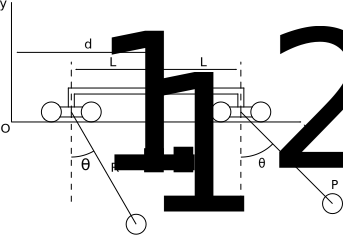
\includegraphics[width=0.5\textwidth]{../../media/cad/sketch.pdf}
    \caption{\textit{Modello del sistema costruito con indicate
     le grandezze rilevanti. Le lettere maiuscole in grassetto indicano dei punti, quelle in corsivo delle 
     costanti; le minuscole invece indicano le variabili.} }
    \label{pendolicorpolibero}
\end{figure}
Innanzitutto consideriamo il diagramma indicato in Fig.\ref{pendolicorpolibero}\footnote{mettere in grassetto i punti, aggiungere l'altezza}.
I tre corpi coinvolti nella dinamica sono i due pendoli, il cui centro 
geometrico è indicato dai punti $\mathbf{P}_1$ e $\mathbf{P}_2$, entrambi di massa $m$,
e il supporto rigido, costituito da due carrellini identici collegati tra loro da un'asta,
indicato dal punto $\mathbf{S}$, arbitrariamente fissato lungo l'asse di simmetria del sistema 
parallelo all'asse $y$, di massa $M$.

Assumiamo che il sistema sia libero di muoversi esclusivamente in un piano fissato, in questo caso
il piano $xy$, e assumiamo che il moto del supporto sia ristretto alla direzione $x$ (è "appoggiato" sull'asse $x$).
Supponiamo che le masse dell'asta e dei fili colleganti i carrellini tra loro
e con le masse oscillanti $\mathbf{P}$ siano trascurabili rispetto alle restanti; 
inoltre trascuriamo anche le masse delle ruote dei carrellini, che, se presenti, si assume ruotino senza strisciare.
Consideriamo le masse dei pendoli puntiformi, fissate nel centro geometrico degli stessi.
In questo modo è possibile ottenere una notevole semplificazione della trattazione analitica,
descrivendo comunque con una buona approssimazione il moto degli elementi principali.

Ricaviamo quindi le coordinate dei tre elementi rilevanti, ossia i due pendoli e il supporto:
$$
\mathbf{P}_1 = (d - L + R \sin \theta_1, A - R \cos \theta_1 ) 
$$
$$
\mathbf{P}_2 = (d + L + R \sin \theta_2, A - R \cos \theta_2 ) 
$$
$$
\mathbf{S} = (d , A) 
$$
Calcoliamo quindi l'energia cinetica per ogni oggetto:
$$
K_{\mathbf{P}_1}=  \frac{m}{2} \lVert \dot{\mathbf{P}}_1 \rVert^2 =  \frac{m}{2}(\dot{d}^2 + R^2 \dot\theta_1^2+ 2\dot{d}R\cos\theta_1 \dot{\theta_1}) 
$$
$$
K_{\mathbf{P}_2} = \frac{m}{2} \lVert \dot{\mathbf{P}}_2 \rVert^2 =  \frac{m}{2}(\dot{d}^2 + R^2 \dot\theta_2^2+ 2\dot{d}R\cos\theta_2 \dot{\theta_2})  
$$
$$
K_{\mathbf{S}} =  \frac{M}{2} \lVert \dot{\mathbf{S}} \rVert^2 = \frac{M}{2} \dot{d}^2
$$
L'energia potenziale invece è:
$$
V_{\mathbf{P}_1}= mg P_{1y} = mg (A - R \cos \theta_1 )
$$
$$
V_{\mathbf{P}_2} = mg P_{2y} = mg (A - R \cos \theta_2 ) 
$$
$$
V_{\mathbf{S}} = mg S_{y} = mgA
$$
E quindi la lagrangiana del sistema si calcola, a meno di costanti, come:
$$
L = K_{TOT} - V_{TOT} = \left(m+ \frac{M}{2}\right) \dot{d}^2 + \frac{m}{2} R^2 (\dot\theta_1^2 + \dot\theta_2^2) + m \dot{d} R (\cos\theta_1 \dot\theta_1 + \cos \theta_2 \dot \theta_2) + mgR(\cos\theta_1 + \cos \theta_2)
$$
\subsection{Equazioni del moto in assenza di attrito}
Approssimiamo ora la lagrangiana considerando il sistema in regime di piccole oscillazioni:
$$
L_{PO} =  \left(m+ \frac{M}{2}\right) \dot{d}^2 + \frac{m}{2} R^2 (\dot\theta_1^2 + \dot\theta_2^2) + m \dot{d} R (\dot \theta_1 + \dot \theta_2) - mgR(\theta_1^2 + \theta_2^2)
$$
Si nota immediatamente che nella lagrangiana è presente una coordinata ciclica, $d$; abbiamo quindi un integrale primo del moto, cioè una quantità che resta costante durante 
l'evoluzione temporale del sistema:
\begin{equation}
p_d = \frac{\partial L_{PO}}{\partial \dot{d}} =(2m+M) \dot d + m R (\dot\theta_1 + \dot \theta_2)
\label{ciclica}
\end{equation}
Sfruttiamo adesso un conveniente cambio di coordinate per gli angoli:
$$ 
\left\{\begin{array}{lr}
  h = \theta_1 + \theta_2 \\
  q = \theta_1 - \theta_2
\end{array}\right.
$$ 
notando che:
$$
  \theta_1^2 + \theta_2^2 = \frac{h^2 +q^2}{2}
$$ 
Le relazioni precedenti valgono anche tra le derivate.
Riscrivendo la lagrangiana otteniamo:
$$
L_{PO} =  \left(m+ \frac{M}{2}\right) \dot{d}^2 + \frac{mR^2}{4}  (\dot{h}^2 + \dot{q}^2) + m  R \dot{d}\dot{h} - \frac{mgR}{2}(h^2 + q^2)
$$
L'Eq.\ref{ciclica} diventa:
\begin{equation}
  p_d = \frac{\partial L_{PO}}{\partial \dot{d}} =(2m+M) \dot d + m R \dot h
  \label{ciclicapost}
\end{equation}
Utilizziamo ora un'altra funzione, la funzione di Routh $R_{PO}$\footnote{mettere la R diversa}, per poter eliminare 
un grado di libertà nelle equazioni del moto. La scriviamo a partire dalla lagrangiana introducendo solamente il
momento $p_d$:
$$
R_{PO}(h,\dot h, q, \dot q, d, p_d )  = 
p_d \dot{d}(p_d, h,\dot h, q, \dot q)- L(h,\dot h, q, \dot q, d, \dot{d}(p_d, h,\dot h, q, \dot q))
$$
dove sono state esplicitate le dipendenze dalle variabili. 
In particolare notiamo che nella lagrangiana dobbiamo scrivere $\dot d$ sfruttando l'Eq.\ref{ciclica}.
Otteniamo quindi:
\begin{equation}
  R_{PO} = \frac{1}{2} \frac{(p_d -mR\dot h)^2}{2m + M}- \frac{mR^2}{4}  (\dot{h}^2 + \dot{q}^2) + \frac{mgR}{2}(h^2 + q^2)
    \label{routh}
\end{equation}
Da questa equazione possiamo ottenere le equazioni del moto, le più importanti sono:
\begin{equation}
  \dot p_d = 0
  \label{conservazione}
\end{equation}
che è coerente con la conservazione di $p_d$ asserita in precedenza, e
\begin{equation}
  \ddot h = -\frac{\alpha}{R} h
\end{equation} 
\begin{equation}
   \ddot q = - \frac{2 g}{R} q
\end{equation}
dove abbiamo usato l'Eq.\ref{conservazione} e posto $\alpha = \frac{2 (2m + M) g}{M} $.
Con queste equazioni a disposizione possiamo completamente ricostruire il moto del sistema.
Notiamo che, partendo da una situazione iniziale arbitraria,
la condizione di sincronizzazione in fase equivale a richiedere che $q$ tenda a zero, mentre quella in controfase
che $h$ tenda a zero. 
Notiamo però che nella soluzione che abbiamo ottenuto una sia $h$ che $q$ descrivono un moto oscillatorio con frequenza rispettiva
$\omega_h = \sqrt[]{\frac{\alpha}{R}}$ e $\omega_q = \sqrt[]{\frac{2g}{R}}$.
Le uniche soluzione per cui i pendoli oscillano sincronizzati sono quelle per cui una tra $h$ o $q$ è nulla
all'inizio del moto, restando quindi nulla per tutti gli istanti successivi.
Il moto evidentemente non converge ad una soluzione particolare, attraversa invece entrambe le configurazioni particolari 
permanendo per il resto degli istante in una combinazione delle due soluzioni.

\subsection{Equazioni del moto in presenza di attrito}
Affinchè il moto converga ad una soluzione particolare, come accade nella realtà, 
è necessario tenere conto dei fenomeni dissipativi.
\begin{comment}
Riscriviamo le due equazioni del moto per $h$ e $q$, sostituendo le vecchie coordinate\footnote{rimettere ref}:
\begin{equation}
  \begin{split}
\ddot \theta_1 + \ddot \theta_2 + \frac{\alpha}{R} (\theta_1 + \theta_2) = 0 \\
\ddot \theta_1 - \ddot \theta_2 + \frac{2g}{R} (\theta_1 - \theta_2) = 0
  \end{split}
  \label{equazionimoto}
\end{equation}
e riorganizzando i termini otteniamo:
\begin{equation}
  \begin{split}
\ddot \theta_1 + \ddot \theta_2 + \frac{\alpha}{R} (\theta_1 + \theta_2) = 0 \\
\ddot \theta_1 - \ddot \theta_2 + \frac{2g}{R} (\theta_1 - \theta_2) = 0
  \end{split}
  \label{equazionimoto}
\end{equation}
\end{comment}
Potremmo ad esempio considerare l'attrito che si sviluppa nel perno 
dei pendoli, quello generato dal movimento delle ruote dei
 carrelli, sia radente che volvente, e quello tra l'aria e le varie 
 componenti mobili.
Supponiamo di voler includere nelle equazioni del moto un termine 
proporzionale alle velocità angolari $\dot \theta_1$ e $\dot \theta_2$, con costante comune di 
proporzionalità $\gamma$, avente le dimensioni di una frequenza. 
Per fare ciò riscriviamo le equazioni del moto 
per queste due variabili, ricavandole dalla $L_{PO}$ e semplificando i fattori in comune:
\begin{equation}
    R \ddot \theta_i + \ddot d = - 2 g  \theta_i ,\qquad \qquad i =1,2
  \label{equazionemotonewton}
\end{equation}
e notiamo che possiamo aggiungere al secondo membro, in cui abbiamo scritto le 
forze generalizzate, l'attrito citato sopra, agente ovviamente in verso 
opposto alla velocità:
\begin{equation}
  R \ddot \theta_i + \ddot d = - 2 g \theta_i  - \gamma   \dot \theta_i,\qquad \qquad i =1,2
  \label{equazionidissipative}
\end{equation}
Scrivendo l'equazione per $d$ possiamo sostituire:
\begin{equation}
  (2m + M) \ddot d = -mR (\ddot \theta_1 + \ddot \theta_2) 
  \label{equazionidissipative}
\end{equation}
Che sostituita nell'equazione precedente dà:
\begin{equation}
  R \ddot \theta_i -\frac{m}{2m + M}R (\ddot \theta_1 + \ddot \theta_2) 
  = - 2 g \theta_i  - \gamma   \dot \theta_i,\qquad \qquad i =1,2
  \label{equazionidissipative}
\end{equation}
che dopo qualche passaggio algebrico possiamo riscrivere con le variabili
$h$ e $q$:
\begin{equation}
  \begin{split}
  (R- \frac{2m}{2m + M}R) \ddot h + \gamma \dot h + 2g h  = 0 \\
  R \ddot q +\gamma \dot q + 2g q = 0 
  \end{split}
  \label{equazionidissipative}
\end{equation}
che tramite una manipolazione algebrica e una ridefinizione di
$\gamma$ diventano:
\begin{equation}
  \begin{split}
  \ddot h + \gamma \dot h + \frac{\alpha}{R} h  = 0 \\
  \ddot q +\gamma \dot q + \frac{2g}{R} q = 0 
  \end{split}
  \label{equazionidissipative}
\end{equation}
La considerazione decisiva per osservare il fenomeno della sincronizzazione 
consiste nel considerare la costante $\gamma$ diversa per i due modi di oscillazione;
differenziando le nuove costanti con un pedice, si tiene conto di 
effetti dissipativi che influenzano in modo differente il modo di oscillazione
in fase rispetto a quello in controfase.
Le soluzioni generali di queste equazioni sono del tipo:
\begin{equation}
    h(t) = A_h e^{- \frac{\gamma_h}{2} t} \cos(\omega_h t + \beta_h)
    \label{equazionefinaleh}
  \end{equation}
    \begin{equation}
    q(t) = A_q e^{- \frac{\gamma_q}{2} t} \cos(\omega_q t + \beta_q)
     \label{equazionefinaleq}
    \end{equation}
con $A_h$, $A_q$, $\beta_h$ e $\beta_q$ costanti reali.
Notiamo quindi che l'ampiezza di uno di questi due modi va a zero più velocemente rispetto 
all'altro, sincronizzando il moto.
\section{Apparato sperimentale}
\subsection{Materiale utilizzato}

Durante l'esperimento sono stati coinvolti diversi elementi, tra cui:
\begin{enumerate}
      \item rotaia e carrellini con basso coefficiente di attrito solitamente
      utilizzati in esperimenti relativi alla conservazione della quantità
      di moto\footnote{Attrezzatura gentilmente concessa dal liceo E.Medi di Senigallia};
      \item due alte sedie in legno;
      \item filo di nylon trasparente;
      \item due strutture identiche progettate autonomamente e stampate in 3D;
      \item scotch di carta;
      \item monete varie;
      \item spago da cucina.
\end{enumerate}

\subsection{Strumenti di misura}

Per quanto riguarda gli strumenti di misura, sono stati invece utilizzati:
\begin{enumerate}
  \item bilancia da cucina;  METTO SENSIBILITA
  \item macchina fotografica semi-professionale;
  \item treppiede per macchina fotografica;
  \item metro estendibile;
  \item libreria di object tracking della suite OpenCV\footnote{https://opencv.org/}.
\end{enumerate}
\subsection{Realizzazione pratica del modello}
Inizialmente la realizzazione del progetto era stata pensata tramite 
una rotaia a cuscino d'aria, idea abbandonata per le numerose difficoltà sperimentali
che avrebbero richiesto troppo tempo per essere risolte.
In seguito si è pensato quindi di utilizzare una semplice rotaia.
La progettazione del modello si è rivolta, una volta recuperata l'apparecchiatura
di laboratorio, alla costruzione dei supporti, disegnati tramite un
software di modellizzazione tridimensionale e stampati con una stampante 3D.
Una volta stampati diversi prototipi e scelto quello migliore sono state incollate
tra loro le due parti costituenti il pezzo finale, e, 
collocato il pezzo sul carrellino, si è costruito il supporto tramite due alte sedie
sopra le quali è stata posta la rotaia. 
È fondamentale sottolineare come si siano scelte le sedie più alte disponibili,
in quanto la lunghezza del pendolo doveva essere grande
per permettere poi l'uso dell'approssimazione di piccole oscillazioni,
non impedendo la chiara manifestazione del fenomeno della sincronizzazione.
È stato controllato che lo sfondo presente dietro le
due sedie fosse inoltre fisso, ossia privo di oggetti
in movimento, per favorire il processo di tracking.
A questo punto sono stati costruiti i due pendoli identici, tramite svariate 
monete raggruppate saldamente insieme grazie all'uso dello scotch di carta, 
pesanti ciascuno $boh$.
Le monete sono state scelte per la loro elevata densità e modularità: è 
stato possibile infatti costrutire diversi pendoli, di dimensioni pressochè
uguali ma di masse sensibilmente diverse gli uni dagli altri.
Sono quindi stati tagliati due pezzi approssimativamente
uguali di filo di nylon, lunghi abbastanza da sfruttare l'intera altezza 
fornita dalle due sedie, e sono poi stati agganciati ai pendoli tramite un pezzo di una nota 
marca di costruzioni giocattolo. Questi due tratti di filo sono stati poi regolati,
con l'ausilio del metro,
tramite la realizzazione di un numero adeguato di avvolgimenti nel perno di 
aggancio.
È importante notare che, per far sì che i pendoli oscillassero nello stesso piano
spaziale per tutta la durata dell'esperimento, i pendoli stessi fossero
liberi di muoversi lungo l'ansa creata dal filo di nylon appeso ai carrellini. 
A questo punto al pendolo di destra è stato collegato un breve tratto di spago 
% dire che si è provato a farlo tutto collegato SCRIVERE DEL FATTO CHE I CARR
% ELLI FOSSERO COLLEGATI
per consentirne la manovra da una posizione che non interferisse con il tracking.
Di fronte a questa apparecchiatura, a una distanza di circa ??? BOH, è stato 
posizionato il treppede con sopra la macchina fotografica, per l'acquisizione
del video.
L'obiettivo della macchina fotografica è stata accuratamente posizionato, per evitare
offset prospettici in un unico verso, su un piano parallelo a quello di oscillazione dei
pendoli e la sua proiezione è stata fatta approssimativamente coincidere con il
centro della circonferenza passante per i due carrellini e i due pendoli a 
riposo.
Infine sono stati acquisiti differenti video del fenomeno, avendo la cura di avere una condizione
iniziale statica, con i tutti gli elementi fermi rispetto al sistema di riferimento della stanza,
con la risoluzione
di 1920 x 1080 pixel, ad un framerate di 25 FPS.

\subsection{Scrittura dei programmi per l'acquisizione e l'elaborazione dati}

Per quanto riguarda la scrittura dei programmi, si è scelto di utilizzare 
la libreria OpenCV, che sta per Open Computer Vision, una libreria open source 
utilizzabile in particolare nei linguaggio di programmazione C++, 
destinata all'analisi di immagini e video. 
In questo esperimento la libreria è stata utilizzata nel per tracciare il 
movimento nel tempo dei pendoli e dei carrellini, in maniera automatizzata.
E' stato utilizzato il C++ per la nota velocità in esecuzione rispetto a 
python. Il codice è listato nell'appendice \ref{listatocpp}.
Il codice inizialmente acquisisce il percorso di memorizzazione del file video, per poi 
permettere all'utente di scegliere prima l'oggetto da tracciare, uno alla volta,
 e poi 
il progressivo dell'acquisizione.
In seguito viene chiesto all'utente di disegnare un rettangolo attorno
all'oggetto di interesse, partendo dal suo centro.
L'algoritmo di tracking, in questo caso KCF\footnote{https://arxiv.org/abs/1404.7584}, 
inizia poi a processare i vari frame, seguendo l'oggetto e scrivendo nel file
le coordinate in pixel del centro del rettangolo (L'origine è nell'angolo in alto a sinistra)
AGGIUNGERE fotografic

. L'utente può e deve fermare l'acquisizione nel caso noti che il rettangolo
scompaia, accompagnato dal messaggio \textit{Tracking failure detected}, relativo al
caso in cui l'algoritmo non riesca a identificare la posizione dell'oggetto
in un determinato frame.

In seguito all'acquisizione di vari set dati, nel nostro caso 4 per ogni oggetto,
per cercare di limitare eventuali errori di posizione, è stata fatta 
una media tramite il programma in Sez.\ref{listatoavg}, stavolta scritto
in python per elasticità nella gestione dei dati in lettura e scrittura.
Sono così stati prodotti quattro files finali, uno per ogni elemento mobile.

Infine, nel listato in Sez.\ref{listatoplotter}, sono stati letti i quattro
files citati sopra, e sono stati poi ricavati con considerazioni
trigonometriche gli angoli indicati in Fig.\ref{pendolicorpolibero} come
$\theta_1$ e $\theta_2$. Sono quindi stati scelti degli intervalli 
temporali appropriati per effettuare i fit di funzioni del tipo \ref{equazionefinaleh} e 
\ref{equazionefinaleq}, in particolare scartando 
i punti iniziali in cui l'apparecchio è fermo, oppure gli ultimi 
qualora il fenomeno da osservare non fosse più presente.

\section{Risultati e discussione}

\begin{figure}[h!]
  \centering
  \includegraphics[width=0.8\textwidth]{../../media/plot/angles_full.pdf}
  \caption{\textit{Modello del sistema costruito con indicate
   le grandezze rilevanti. Le lettere maiuscole in grassetto indicano dei punti, quelle in corsivo delle 
   costanti; le minuscole invece indicano le variabili.} }
  \label{angles_full}
\end{figure}

\begin{figure}[h!]
  \centering
  \includegraphics[width=0.8\textwidth]{../../media/plot/angles_accurate.pdf}
  \caption{\textit{Modello del sistema costruito con indicate
   le grandezze rilevanti. Le lettere maiuscole in grassetto indicano dei punti, quelle in corsivo delle 
   costanti; le minuscole invece indicano le variabili.} }
  \label{anlges_accurate}
\end{figure}

\begin{figure}[h!]
  \centering
  \includegraphics[width=0.8\textwidth]{../../media/plot/fit_h.pdf}
  \caption{\textit{Modello del sistema costruito con indicate
   le grandezze rilevanti. Le lettere maiuscole in grassetto indicano dei punti, quelle in corsivo delle 
   costanti; le minuscole invece indicano le variabili.} }
  \label{fit_h}
\end{figure}

\begin{figure}[h!]
  \centering
  \includegraphics[width=0.8\textwidth]{../../media/plot/fit_q.pdf}
  \caption{\textit{Modello del sistema costruito con indicate
   le grandezze rilevanti. Le lettere maiuscole in grassetto indicano dei punti, quelle in corsivo delle 
   costanti; le minuscole invece indicano le variabili.} }
  \label{fit_q}
\end{figure}

\begin{figure}[h!]
  \centering
  \includegraphics[width=0.8\textwidth]{../../media/plot/angles_decrease.pdf}
  \caption{\textit{Modello del sistema costruito con indicate
   le grandezze rilevanti. Le lettere maiuscole in grassetto indicano dei punti, quelle in corsivo delle 
   costanti; le minuscole invece indicano le variabili.} }
  \label{angles_decrease}
\end{figure}



RIORDINARE Q E H 


\section{Appendice}
Nei seguenti listati sono presenti i file con i quali sono stati estratti 
e visualizzati i dati dell'esperimento.
\subsection{Listato del programma di tracking (C++)}
\lstinputlisting[language=C++]{../c++/tracking.cpp}
\label{listatocpp}
\subsection{Listato del programma di elaborazione dei dati (python)}
\lstinputlisting[language=Python]{../python/avg.py}
\label{listatoavg}
\subsection{Listato del programma di fit e visualizzazione dati (python)}
\lstinputlisting[language=Python]{../python/plotter.py}
\label{listatoplotter}

\end{document}
